\documentclass[a4paper,10pt]{ltjsarticle}

\usepackage{setspace}

\usepackage{comment} 
\usepackage{substr}
\setcounter{secnumdepth}{4}

\usepackage{graphicx} 
\usepackage{float} 

% LINK
\usepackage{url}
\usepackage{hyperref}
\hypersetup{pdfborder={0 0 0.5}}

% 色の使用
\usepackage{xcolor}
% 色定義
\definecolor{mylinkcolor}{RGB}{3, 112, 145}
\definecolor{clBlue}{RGB}{3, 112, 145}
\definecolor{linkcol}{RGB}{2, 106, 77}
\definecolor{rred}{RGB}{128, 0, 0}
\hypersetup{
    colorlinks=true,
    citecolor=blue,
    linkcolor=linkcol, 
    urlcolor=mylinkcolor
}
% HTML(#800000)色定義
\def\colH#1{\color[HTML]{#1}}

% FONT-SIZE 定義
\def\fs#1{\fontsize{#1}{#1}\selectfont }
% BACKSLASH 定義
\def\bs{\textbackslash }

% \setlength\parindent{0pt} % 段落はじめの空白を除去

% FONT 
\usepackage{luatexja-otf}% UTF CID
\usepackage[deluxe]{luatexja-preset}
\usepackage{luatexja-fontspec}

% 縦組
\usepackage{lltjext}

\usepackage{./lib/lib-russian-luatexja} 
\ltjdefcharrange{8}
{
"2626-"262E
%,"E000-"EDEA,"F340-"FE2F,"2E2A-"2E43,"10FB-"1DC1 % 記号:☦ ☩ ☪ ☫ ☬ ☭ ☮
}


\def\basefont{NotoSerifCJKjp-Regular} 
\setmainfont{\basefont} 
% フォント名
\def\myMainfont{
  \BeforeSubString{-Regular}{\basefont}
}
\setsansfont{NotoSans}
\setmonofont{RobotoMono-Light}% NotoSansMono

% 
% フォントの定義設定
% 
\newfontfamily\fTimes{times}
\newfontfamily\fArial{arial}
\newfontfamily\fFSerif{FreeSerif}
\newfontfamily\fRoboto{roboto}
\newfontfamily\fYumin{yumin}
\newfontfamily\fIPAM{HaranoAjiMincho-Regular}
\newfontfamily\fNCMSans{NewCMSans10-Regular}
\newfontfamily\fCRoman{Crimson-Roman}
\newfontfamily\fDjVSerif{DejaVuSerif}
\newfontfamily\fDjVSans{DejaVuSans}

\newfontfamily\chIrmIEUcs{IrmIEUcs}

%%
%% キリル文字フォント用の設定
%%
\newfontfamily\cyrillicfontsf[Script=Cyrillic,Ligatures=TeX]{PomorskyUnicode}%FreeSerif
\newfontfamily\cyrillicfonttt[Ligatures=TeX]{PomorskyUnicode}
\newfontfamily\russianfont[Script=Cyrillic,Ligatures=TeX]{Linux Libertine O}
\newfontfamily\russianfonttt[Ligatures=TeX]{lmmono10-regular.otf}
\newfontfamily\russianfontsf[Ligatures=TeX]{lmsans10-regular.otf}
\newfontfamily\churchslavonicfont[Script=Cyrillic,Ligatures=TeX,HyphenChar=_]{PonomarUnicode.otf}

%%
%% fonts-churchslavonic:教会スラヴ語フォントの定義
%% /usr/share/texlive/texmf-dist/fonts/opentype/public/fonts-churchslavonic
\newfontfamily\Acathist[Script=Cyrillic,Ligatures=TeX]{Acathist-Regular.otf}
\newfontfamily\Cathisma[Script=Cyrillic,Ligatures=TeX]{CathismaUnicode.otf}
\newfontfamily\Fedorovsk[Script=Cyrillic,Ligatures=TeX]{FedorovskUnicode.otf}
\newfontfamily\Indiction[Script=Cyrillic,Ligatures=TeX]{IndictionUnicode.otf}
\newfontfamily\Menaion[Script=Cyrillic,Ligatures=TeX]{MenaionUnicode.otf}
\newfontfamily\MezenetsNo[Script=Cyrillic,Ligatures=TeX]{MezenetsUnicode.otf}
\newfontfamily\Mezenets[Script=Cyrillic,Ligatures=TeX]{MezenetsUnicode.otf}
\newfontfamily\Monomakh[Script=Cyrillic,Ligatures=TeX]{MonomakhUnicode.otf}
\newfontfamily\Oglavie[Script=Cyrillic,Ligatures=TeX]{OglavieUnicode.otf}
\newfontfamily\Pochaevsk[Script=Cyrillic,Ligatures=TeX]{PochaevskUnicode.otf}
\newfontfamily\Pomorsky[Script=Cyrillic,Ligatures=TeX]{PomorskyUnicode.otf}
\newfontfamily\Ponomar[Script=Cyrillic,Ligatures=TeX]{PonomarUnicode.otf}
\newfontfamily\Shafarik[Script=Cyrillic,Ligatures=TeX]{Shafarik-Regular.otf}
\newfontfamily\Triodion[Script=Cyrillic,Ligatures=TeX]{TriodionUnicode.otf}
\newfontfamily\Vertograd[Script=Cyrillic,Ligatures=TeX]{VertogradUnicode.otf}

% 
% SECTIONの定義
% 
\usepackage{titlesec}
\titleformat{\section}[block]{\gtfamily \large}{\thesection}{0.5em}{}% 
\titleformat{\subsection}[block]{\gtfamily \large}{\thesubsection}{0.5em}{}% 

% 
% BibLaTeX
% 
\usepackage[
  backend=biber,
  bibstyle=ieee,
]{biblatex}
\nocite{*}
\addbibresource{./lib/sample.bib} % .bibデータの読込
\renewcommand{\bibfont}{\fFSerif}
%  [Online]. Available => URL
\DeclareFieldFormat{url}{\mkbibacro{参照}{\Large\addcolon}\space\url{#1}}
% URL FONT
\def\UrlFont{\normalfont}
% author name: 
\renewcommand{\labelnamepunct}{\Large\addcolon\space}


\usepackage{listings}
\usepackage{tablefootnote}

% TITLEPAGE 
\title{
  \huge Template of Russian Typesetting\\ on LuaTeX-ja\vspace{16mm} \par
  \Large{ロシア語資料の作成}\vspace{6mm}\\
  \small{基本フォント: \myMainfont 版}
\par\vspace{120mm}
}
\author{\href{https://github.com/ru-museum/}{ru\_museum} (GitHub)}
\date{\today}


\begin{document}

\maketitle

\thispagestyle{empty}
\clearpage

\newpage

{\makeatletter
\let\ps@jpl@in\ps@empty
\makeatother
\pagestyle{empty}
\tableofcontents
\clearpage}

  
% \tableofcontents
% \thispagestyle{empty}

\newpage
% \clearpage
\addtocounter{page}{-3}

\section{概要}
これは、日本語文書組版パッケージ \textbf{\colH{800000} LuaTeX-ja} での環境 ( \textbf{\colH{800000} ltjsclasses}\footnote{jsclasses を LuaTeX-ja 用に改変したもの。ltjsarticle 他がある。} ) において和露混在文を作成する為のロシア語の記述方法を解説するものです。\vspace{6pt}\\
基本を和文フォントとする LuaTeX-ja 環境では、ロシア及びギリシア文字は和文フォントに割り振られている為に\textbf{等幅表示}されることからプロポーショナル表記に難があり、単語のハイフネーションや禁則処理に乱れを生じます。\vspace{6pt}\par

そうした問題を解消し、ロシア語の\textbf{プロポーショナル表記}を可能としています。\vspace{6pt}\par

従来LaTeX{}では多言語混在の文書作成にはp\LaTeX{} 由来の class \textbf{"article"}と\textbf{Babel}の組み合わせ、更にはその代替の\textbf{Polyglossia}が用いられて来ています。\vspace{6pt}\par

LuaTeX-ja(ltjsarticle等)環境においてもそれら両者を使用することは出来ますが、基本を和文フォントとする以上問題は解決されません。\vspace{6pt}\par

以下の表示例に示す様に、それらを使用せず和露混在文\footnote{特別にフォントを指定し字体を変える以外にはロシア語への特別なマークアップは必要ありません。}を自由に編集出来ます。\vspace{-2mm}\par

\vspace{6pt}
\begin{table}[h]
\begin{center}
\begin{tabular}{l|l}
\textbf{和露混在文} & \textbf{指定フォント}\\
\hline
これは{\color[HTML]{800000}\fIPAM Л. Н. Толстой}テストです。 & IPAex明朝\tablefootnote{「IPAフォント」をベースにした「IPAexフォント」は、「和文の文字を固定幅、欧文の文字をプロポーショナルで表示するTrueTypeフォント」と謳っていますがキリル文字には対応していない様です。}(IPA P明朝)、原ノ味\\
これは{\color[HTML]{800000}Л. Н. Толстой}テストです。 &  \basefont(default)\\
これは{\color[HTML]{800000}\fTimes{ Л. Н. Толстой}}テストです。 & Times(PSCyr)\\
これは{\color[HTML]{800000}\fArial{ Л. Н. Толстой}}テストです。 & Arial(PSCyr)\\
\end{tabular}
\caption{表示例}
\end{center}
\end{table}
\vspace{-6mm}

\section{環境構築}

\begin{itemize} 
  \item ここではGNU/Linux Debian (sid) での使用例です。
  \item Babel 及び Polyglossia は使用しません。\vspace{-2mm}
\end{itemize}

\subsection{インストールパッケージ}
\vspace{-2mm}
\begin{quote}
\begin{verbatim}
texlive-base v. 2022.20230122-3(sid)  
texlive-luatex
texlive-lang-japanese(LuaTeX-ja)
texlive-lang-cyrillic(ロシア語フォント、Polyglossia等)
\end{verbatim}\vspace{-4mm}
\end{quote}

\subsection{和文フォント}

\begin{itemize} 
  \item 現在プロポーショナル\footnote{「等幅」を欧文フォントのプロポーショナル化する処理。}に対応し無料で入手可能で、問題の生じない推奨和文フォントには主に以下のものがあります。 ⇒参照:「3.2.1 基本フォントの指定 表3 基本設定に適する主要フォント」  
  \vspace{-8mm}\\
\begin{quote}
\begin{table}[h]
\begin{center}
\begin{tabular}{l|l}
\textbf{対応和文フォント} & \textbf{フォント名}\\
\hline\vspace{-4mm}\\
\href{https://fonts.google.com/noto/specimen/Noto+Serif+JP}{NotoSerifJP} & Noto Serif Japanese(Google Fonts)\\
 & {\fs{9}//fonts.google.com/noto/specimen/Noto+Serif+JP}\\
\href{https://github.com/notofonts/noto-cjk}{NotoSerifCJK} &  Noto CJK fonts(GitHub)\\
 & {\fs{9}//github.com/notofonts/noto-cjk}\\
\href{https://github.com/adobe-fonts/source-serif/tree/release/OTF}{SourceSerif4} & Source Serif(adobe-fonts/GitHub)\\
 & {\fs{9}//github.com/adobe-fonts/source-serif/tree/release/OTF}\\
\href{https://github.com/IBM/plex/tree/master/IBM-Plex-Serif/fonts/complete/otf}{IBMPlexSerif} & IBM Plex typeface(GitHub)\\ 
 & {\fs{9}//github.com/IBM/plex/tree/master/IBM-Plex-Serif/fonts/complete/otf}\\
\end{tabular}
\caption{主要和文フォント}\vspace{-2mm}
\end{center}
\end{table}
\end{quote} 
\end{itemize} 

\subsection{欧文フォント(PSCyr)}

\begin{itemize} 
  \item Linux及びTexLiveには所謂Windows系のTimes New RomanやArial系の欧文書体はインストールされていません。ここではTimesやArial系が同梱されたPSCyrパッケージを以下のHPからダウンロードします。\\ 
  \href{http://tex.imm.uran.ru/texserver/fonts/pscyr/pscyr4c/}{TeX в ИММ}\\
  {\fs{11}http://tex.imm.uran.ru/texserver/fonts/pscyr/pscyr4c/}\\  
  \href{http://tex.imm.uran.ru/texserver/fonts/pscyr/PSCyr-0.4c-patch2-type1.tar.gz}{PSCyr-0.4-type1.tar.gz}\\
  {\fs{11}http://tex.imm.uran.ru/texserver/fonts/pscyr/PSCyr-0.4c-patch2-type1.tar.gz}\\
\href{https://ctan.org/topic/font-otf}{OTF Font} (CTAN: OpenType/TrueTypeの欧文フォントがダウンロード可能)\\
https://ctan.org/topic/font-otf
\end{itemize}
\vspace{-2mm}

\subsection{フォントのインストール}
\begin{itemize}
  \item インストールするフォルダの位置は環境により異なります。\vspace{-4mm}
\end{itemize}

\subsubsection{PSCyrパッケージのインストール}

\vspace{2mm}

\begin{enumerate}
  \item 解凍したPSCyrパッケージのフォルダ構成は以下の様になっています。
{\fs{10pt}
\begin{verbatim}
 ├fonts
    ├afm
    └type1
       └public
         └pscyr
           ├acade1.pfb
           ├・・・・・
           └timesi.pfb
\end{verbatim}
}

  \item /type1/public/内のフォルダpscyr以下をコピーし、\\
  /usr/share/texlive/texmf-dist/fonts/type1/public内に貼り付けます。\\
/usr/share/texlive/texmf-dist/fonts/type1/public/{\colH{800000} pscyr/*.pfb}
\end{enumerate}

\subsubsection{和文フォントのインストール}

\begin{enumerate}
  \item OTFのフォントは/opentype或いは/opentype/publicフォルダへ追加します。\\
【インストール例】\\
/usr/share/texlive/texmf-dist/fonts/opentype/adobe/sourcehanserif/*.otf\\
/usr/share/texlive/texmf-dist/fonts/opentype/google/noto/*.otf  
  \item OS付属の/usr/share/fontsにある各種フォントも基本的に使用可能です。\vspace{-2mm}
\end{enumerate}

\section{作成手順}

\subsection{ライブラリーの読込}
{\colH{800000} lib-russian-luatexja.sty} パッケージを読込みます。
\vspace{-2mm}
\begin{verbatim}
  \usepackage[deluxe]{luatexja-preset} % 必須
  \usepackage{./lib/lib-russian-luatexja} 
\end{verbatim}
\vspace{-6mm}
    
\subsection{フォントの設定と定義}

\subsubsection{基本フォントの指定}
\begin{itemize}
  \item[]\hspace{-5mm} {\colH{800000}\bs setmainfont\{} \basefont{\colH{800000} \}}
  \item 基本指定した書体の和文フォントは全体に適用されます。
  \item 特に指定がなければTexLiveのデフォルトのHarano Aji Fonts(haranoaji)が設定されます。
  \item 現在適正に表記の出来る\textbf{主な基本設定向けフォント}は以下のものがあります。\\
  インストール方法は 「\fRoboto{2.4} {\textbf フォントのインストール}」を参照して下さい。\vspace{-4mm}
\end{itemize}
\begin{table}[h]
\begin{center}
\begin{tabular}{l|c|l}
\textbf{フォント名} & \textbf{提供元} & \textbf{用途}\\
\hline
NotoSerifCJKjp-Regular & Google & 和文\\%
NotoSerifJP-Regular & Google & 和文\\%
SourceSerif4-Regular & Adobe & 和文\\%
SourceSerifJP-Regular & Adobe & 和文\\%
SourceHanSerif-Regular & Adobe & 和文\\%
SourceHanSans-Regular & Adobe & 和文\\%
IBMPlexSerif-Regular & IBM & 和文\\%
RobotoSlab-Regular & Google & 欧文\\%
roboto & Google & 欧文\\%
times, arial etc. & PSCyr & 欧文\\%
RobotoSlab-Regular & Google & 欧文\\%
NewCMSans10-Regular & TexLive & 欧文\\%
CMU Serif, CMU Sans & TexLive & 欧文\\%
FreeSerif, FreeSans & TexLive & 欧文\\%
\end{tabular}
\caption{基本設定に適する主要フォント}
\end{center}
\end{table}

\subsubsection{個別フォントの定義}
\begin{itemize}
  \item[] {\colH{800000} \textbackslash newfontfamily\textbackslash<command>\{<fontname>\}}
\vspace{-2mm}
\begin{verbatim}
定義例:\newfontfamily\fArial{arial}
       \newfontfamily\fRoboto{roboto} % Google OTF
\end{verbatim} 
\vspace{-2mm}
  \item <command>名は自由に宣言出来ます。  
  \item インストールされているフォントを確認し試行を行って下さい。\\
OS(Debian): /usr/share/fonts/\\
TexLive: /usr/share/texlive/texmf-dist/fonts/\vspace{-4mm}
\end{itemize}

\subsubsection{混在文におけるフォント指定}
\begin{itemize}
  \item 定義したフォントを指定したい文字列へ適用します。
  \item[] {\colH{800000} \textbackslash <command>\{<text>\}}
  \item[] \textbf{記述例}:ロシアの作家 {\colH{800000}\textbackslash fTimes\{}Толстой{\colH{800000}\}} と {\colH{800000}\textbackslash fArial\{}Достоевский{\colH{800000}\}} は思想家でもある。\vspace{2mm}\\
    \textbf{表示結果}:ロシアの作家\fTimes{Толстой}と\fArial{Достоевский}は思想家でもある。
% \vspace{6mm}
\end{itemize}

\section{指定フォントによる表示例}
\subsection{基本フォント: \textcolor{rred}{NotoSerifCJKjp-Regular}(地文)}

\begin{itemize} 
  \item[]
\textbf{和文}\\
\hspace{3mm} 日本国民は正当に選挙された国会における代表者を通じて行動し、われらとわれらの子孫のために、諸国民と協和による成果と、わが国全土にわたって自由のもたらす恵沢を確保し、政府の行為によって再び戦争の惨禍が起こることのないようにすることを決意し、ここに主権が国民に存することを宣言し、この憲法を確定する。そもそも国政は国民の厳粛な信託によるものであって、その権威は国民に由来し、その権力は国民の代表者がこれを行使し、その福利は国民がこれを享受する。これは人類普遍の原理であり、この憲法は、かかる原理に基づくものである。われらはこれに反する一切の憲法、法令及び詔勅を排除する。\par

\hspace{3mm} 日本国民は、恒久の平和を念願し、人間相互の関係を支配する崇高な理想を深く自覚するのであって、平和を愛する諸国民の公正と信義を信頼して、われらの安全と生存を保持しようと決意した。われらは平和を維持し、専制と隷従、圧迫と偏狭を地上から永遠に除去しようと努めている国際社会において、名誉ある地位を占めたいと思う。われらは全世界の国民が、ひとしく恐怖と欠乏から免れ、平和の内に生存する権利を有することを確認する。\par

\hspace{3mm} われらは、いずれの国家も、自国のことのみに専念して他国を無視してはならないのであって、政治道徳の法則は、普遍的なものであり、この法則に従うことは、自国の主権を維持し、他国と対等関係に立とうとする各国の責務であると信ずる。\par

日本国民は、国家の名誉にかけて、全力をあげて崇高な理想と目的を達成することを誓う。\footnote{「日本国憲法」 前文}
 \par 

\newpage

\textbf{英文}\\
\hspace{3mm} Lorem ipsum dolor sit amet, consectetur adipiscing elit, sed do eiusmod tempor inincididunt ut labore et dolore magna aliqua. Ut enim ad minim veniam, quis nostrud exercitation ullamco laboris nisi ut aliquip ex ea commodo consequat.\vspace{2mm}
\par
  \item[]
\textbf{露文}\\
\hspace{3mm}Все счастливые семьи похожи друг на друга, каждая несчастливая семья несчастлива по-своему.\par
\hspace{3mm}Всё смешалось в доме Облонских. Жена узнала, что муж был в связи с бывшею в их доме Француженкою-гувернанткой, и объявила мужу, что не может жить с ним в одном доме. Положение это продолжалось уже третий день и мучительно чувствовалось и самими супругами, и всеми членами семьи, и домочадцами. Все члены семьи и домочадцы чувствовали, что нет смысла в их сожительстве и что на каждом постоялом дворе случайно сошедшиеся люди более связаны между собой, чем они, члены семьи и домочадцы Облонских. Жена не выходила из своих комнат, мужа третий день не было дома. Дети бегали по всему дому, как потерянные; Англичанка поссорилась с экономкой и написала записку приятельнице, прося приискать ей новое место; повар ушел еще вчера со двора, во время обеда; черная кухарка и кучер просили расчета.\par
\hspace{3mm} На третий день после ссоры князь Степан Аркадьич Облонский — Стива, как его звали в свете, — в обычайный час, то есть в 8 часов утра, проснулся не в спальне жены, а в своем кабинете, на сафьянном диване. Он повернул свое полное, выхоленное тело на пружинах дивана, как бы желая опять заснуть надолго, с другой стороны крепко обнял подушку и прижался к ней щекой; но вдруг вскочил, сел на диван и открыл глаза.\par 
\hspace{80mm}— Анна Каренина: Л. Н. Толстой\footnote{Анна Каренина: Л. Н. Толстой, Полное собрание сочинений. Том 18, Часть Первая. I. с.3\\
https://tolstoy.ru/upload/iblock/a58/18\_tom.pdf // Льв Толстой(Tolstoy.ru)}
\end{itemize}

\subsection{指定フォント: \textcolor{rred}{Times}}
\fTimes{
\setlength{\leftskip}{10mm}
Все счастливые семьи похожи друг на друга, каждая несчастливая семья несчастлива по-своему.\par
Всё смешалось в доме Облонских. Жена узнала, что муж был в связи с бывшею в их доме Француженкою-гувернанткой, и объявила мужу, что не может жить с ним в одном доме. Положение это продолжалось уже третий день и мучительно чувствовалось и самими супругами, и всеми членами семьи, и домочадцами. Все члены семьи и домочадцы чувствовали, что нет смысла в их сожительстве и что на каждом постоялом дворе случайно сошедшиеся люди более связаны между собой, чем они, члены семьи и домочадцы Облонских. Жена не выходила из своих комнат, мужа третий день не было дома. Дети бегали по всему дому, как потерянные; Англичанка поссорилась с экономкой и написала записку приятельнице, прося приискать ей новое место; повар ушел еще вчера со двора, во время обеда; черная кухарка и кучер просили расчета.\par
На третий день после ссоры князь Степан Аркадьич Облонский — Стива, как его звали в свете, — в обычайный час, то есть в 8 часов утра, проснулся не в спальне жены, а в своем кабинете, на сафьянном диване. Он повернул свое полное, выхоленное тело на пружинах дивана, как бы желая опять заснуть надолго, с другой стороны крепко обнял подушку и прижался к ней щекой; но вдруг вскочил, сел на диван и открыл глаза.\par 
\hspace{80mm}— Анна Каренина: Л. Н. Толстой}

\subsection{指定フォント: \textcolor{rred}{Arial}}
\fArial{
\setlength{\leftskip}{10mm}
Все счастливые семьи похожи друг на друга, каждая несчастливая семья несчастлива по-своему.\par
Всё смешалось в доме Облонских. Жена узнала, что муж был в связи с бывшею в их доме Француженкою-гувернанткой, и объявила мужу, что не может жить с ним в одном доме. Положение это продолжалось уже третий день и мучительно чувствовалось и самими супругами, и всеми членами семьи, и домочадцами. Все члены семьи и домочадцы чувствовали, что нет смысла в их сожительстве и что на каждом постоялом дворе случайно сошедшиеся люди более связаны между собой, чем они, члены семьи и домочадцы Облонских. Жена не выходила из своих комнат, мужа третий день не было дома. Дети бегали по всему дому, как потерянные; Англичанка поссорилась с экономкой и написала записку приятельнице, прося приискать ей новое место; повар ушел еще вчера со двора, во время обеда; черная кухарка и кучер просили расчета.\par
На третий день после ссоры князь Степан Аркадьич Облонский — Стива, как его звали в свете, — в обычайный час, то есть в 8 часов утра, проснулся не в спальне жены, а в своем кабинете, на сафьянном диване. Он повернул свое полное, выхоленное тело на пружинах дивана, как бы желая опять заснуть надолго, с другой стороны крепко обнял подушку и прижался к ней щекой; но вдруг вскочил, сел на диван и открыл глаза.\par 
\hspace{80mm}— Анна Каренина: Л. Н. Толстой}\vspace{-2mm}

\subsection{指定フォント: \textcolor{rred}{roboto}}
\fRoboto{
\setlength{\leftskip}{10mm}
Все счастливые семьи похожи друг на друга, каждая несчастливая семья несчастлива по-своему.\par
Всё смешалось в доме Облонских. Жена узнала, что муж был в связи с бывшею в их доме Француженкою-гувернанткой, и объявила мужу, что не может жить с ним в одном доме. Положение это продолжалось уже третий день и мучительно чувствовалось и самими супругами, и всеми членами семьи, и домочадцами. Все члены семьи и домочадцы чувствовали, что нет смысла в их сожительстве и что на каждом постоялом дворе случайно сошедшиеся люди более связаны между собой, чем они, члены семьи и домочадцы Облонских. Жена не выходила из своих комнат, мужа третий день не было дома. Дети бегали по всему дому, как потерянные; Англичанка поссорилась с экономкой и написала записку приятельнице, прося приискать ей новое место; повар ушел еще вчера со двора, во время обеда; черная кухарка и кучер просили расчета.\par
На третий день после ссоры князь Степан Аркадьич Облонский — Стива, как его звали в свете, — в обычайный час, то есть в 8 часов утра, проснулся не в спальне жены, а в своем кабинете, на сафьянном диване. Он повернул свое полное, выхоленное тело на пружинах дивана, как бы желая опять заснуть надолго, с другой стороны крепко обнял подушку и прижался к ней щекой; но вдруг вскочил, сел на диван и открыл глаза.\par 
\hspace{80mm}— Анна Каренина: Л. Н. Толстой
}

\subsection{指定フォント: \textcolor{rred}{FreeSerif}}
\fFSerif{
\setlength{\leftskip}{10mm}
Все счастливые семьи похожи друг на друга, каждая несчастливая семья несчастлива по-своему.\par
Всё смешалось в доме Облонских. Жена узнала, что муж был в связи с бывшею в их доме Француженкою-гувернанткой, и объявила мужу, что не может жить с ним в одном доме. Положение это продолжалось уже третий день и мучительно чувствовалось и самими супругами, и всеми членами семьи, и домочадцами. Все члены семьи и домочадцы чувствовали, что нет смысла в их сожительстве и что на каждом постоялом дворе случайно сошедшиеся люди более связаны между собой, чем они, члены семьи и домочадцы Облонских. Жена не выходила из своих комнат, мужа третий день не было дома. Дети бегали по всему дому, как потерянные; Англичанка поссорилась с экономкой и написала записку приятельнице, прося приискать ей новое место; повар ушел еще вчера со двора, во время обеда; черная кухарка и кучер просили расчета.\par
На третий день после ссоры князь Степан Аркадьич Облонский — Стива, как его звали в свете, — в обычайный час, то есть в 8 часов утра, проснулся не в спальне жены, а в своем кабинете, на сафьянном диване. Он повернул свое полное, выхоленное тело на пружинах дивана, как бы желая опять заснуть надолго, с другой стороны крепко обнял подушку и прижался к ней щекой; но вдруг вскочил, сел на диван и открыл глаза.\par 
\hspace{80mm}— Анна Каренина: Л. Н. Толстой
}

\section{ロシア語翻字}

\begin{itemize}
  \item ロシア語翻字\footnote{ロシア語と翻字(ローマ字)との相互変換は、\href{https://www.art-russian.org/}{ロシア美術資料館}で提供しています(https://www.art-russian.org/)。}を表記するには、収録されているフォントを指定する必要があります。
  \item 現在適正表記の出来るフォントには{\colH{800000}DejaVuSans}\footnote{DejaVuSerifは不可。}、{\colH{800000}FreeSerif}、{\colH{800000}FreeSans}\footnote{gnu-freefontとしてTexLiveによりデフォルトでインストールされています。\\/usr/share/texlive/texmf-dist/fonts/opentype/public/gnu-freefont/Free*.otf}等があります。
\vspace{-2mm}
\begin{table}[h]
\begin{center}
\begin{tabular}{l|l|l}
\textbf{文字化け} & \textbf{正常表記(FreeSerif)}& \textbf{記述例}\\
\hline
\fDjVSerif{Evgeni{\colH{800000}i︠a︡ }Andreevna} & \fFSerif{Evgeni{\colH{800000}i︠a︡ } Andreevna} & {\colH{800000}\bs fFSerif}\{\fFSerif{Evgenii︠a︡  Andreevna}\}\\
\end{tabular}
\caption{翻字表記と記述例}
\end{center}
\end{table}\vspace{-6mm}

  \item BibLaTeX内での翻字表記については特別な対処が必要です。\\
  詳しくは\textbf{\gtfamily 10.4 BibLaTeX内での翻字表記}を参照して下さい。
\end{itemize}


\section{教会スラブ語(Church Slavonic)}

\begin{itemize}
  \item 教会スラブ語の表記も可能です。\\
 \verb+\usepackage{churchslavonic}+

\textbf{表記例:}\\
\Monomakh{Хрⷭ҇то́съ воскре́се и҆з̾ ме́ртвыхъ, сме́ртїю сме́рть попра́въ, и҆ сꙋ́щымъ во гробѣ́хъ живо́тъ дарова́въ.\\
Послѣ́дованїе моле́бнагѡ пѣ́нїѧ ст҃ ы̑ мъ мч҃ камъ к҃ \_гѡ вѣ́ка, въ Са́нктъ\_
Петербꙋр́ жстѣй дꙋхо́внѣй а҆каде́мїи нача̑льствовавшимъ, ᲂу҆ чи̑ вшимъ и҆ ᲂу҆
чи̑ вшимсѧ}

  \item 詳しくはこちらに解説しています。\\
  \href{https://github.com/ru-museum/lib-russian-luatexja/blob/main/churchslavonic-luatexja.pdf}{教会スラヴ語:Church Slavonic Typesetting in LuaTeX-ja}(churchslavonic-luatexja.pdf)
\end{itemize}\vspace{-4mm}

\section{特別な文字・記号の表記}

\subsection{記号の表記方法}\vspace{-2mm}

\begin{itemize}
  \item フォントビューワーで使用する記号及びUnicode番号を調べます(参照:\textbf{12 付録:Cyrillic Unicode 表})。\\[-14pt] 
\begin{figure}[H]
\centering
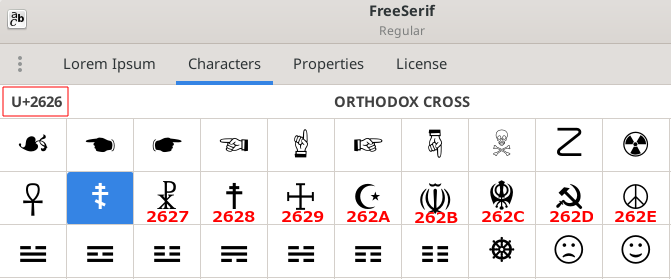
\includegraphics[width=12cm]{./images/unicode.png}  
\caption{記号のUnicode番号} 
\end{figure}
\vspace{-6mm}
  \item[] \textbf{方法1}:直接記号を記述する。\\[-12pt]
\begin{quote}
  \textbf{記述例:}\verb+{\jfontspec{FreeSerif} +{\jfontspec{FreeSerif}\fs{12}☦☭☁☂☃☇☠♁♂♃♄♅}\verb+}+\\
  \textbf{表示例:}{\jfontspec{FreeSerif}\fs{14}☦☭☁☂☃☇☠♁♂♃♄♅}\\[-10pt]
  \end{quote}

  \item[] \textbf{方法2}:Unicodeで指定し記述する。\\[-12pt]
\begin{quote}
\verb+\UTF{<unicode>}+ \% \verb+\usepackage{luatexja-otf}+ が必要\\
\textbf{記述例:}\vspace{-11.2mm}\\
\begin{verbatim}
      {\jfontspec{FreeSerif} \UTF{2626}\UTF{2627}\UTF{2628}
                             \UTF{2629}\UTF{262A}\UTF{262B}
                             \UTF{262C}\UTF{262D}\UTF{262E}}
\end{verbatim} 
  \textbf{表示例:}{\jfontspec{FreeSerif}\fs{14}
      \UTF{2626}\UTF{2627}\UTF{2628}\UTF{2629}
      \UTF{262A}\UTF{262B}\UTF{262C}\UTF{262D}\UTF{262E}}
\end{quote}
  
  \item[] \textbf{方法3}:個々の文字・記号或いは範囲を指定する。\footnote{この場合直接記述或いは \bs jfontspecで記述出来ますが、TABLE内等の閉じられた環境に依っては \bs fontspecで指定しないとエラーとなります。}
\begin{quote}
   例:"2626-"262E(☦ ☩ ☪ ☫ ☬ ☭ ☮) 
\begin{verbatim}
\ltjdefcharrange{8}{ "2626,"2627-"262E }
\end{verbatim}
\end{quote}
\end{itemize}

\section{縦組におけるロシア語}

\begin{minipage}{8cm}
\begin{itemize}
  \item 全体の縦組用classにはltj{\colH{800000}t}article、ltj{\colH{800000}t}book等が用意されています。
  \item 縦中横など異方向の混在には、各々{\colH{800000}\verb|\tate|}、{\colH{800000}\verb|\yoko|}のプリミティブを使用します。
  \item 連数字(\verb|\rensuji{<num>}|)を用いるには、\verb|\usepackage{lltjext}|が必要です。
  \item 表記例先頭の「縦向きロシア文字」表記には、連数字用の\verb|\rensuji{|{\colH{800000}Л}\verb|}|を代用します。\\
  頭字語(МХАТなど)の単語にもこれを用います。
\end{itemize}
\end{minipage}

\vspace{-56mm}\hspace{90mm}
\vbox{\hsize=60mm\raggedright%left
\tate \rensuji{\colH{800000}Л}・\rensuji{\colH{800000}Н}・トルストイは1901年、宗務院より教会破門の宣告を受けた。そしてトルストイ({\colH{800000}Л. Н. Толстой})は\rensuji{10}年、予てからの思想上の苦悩と妻との生活上の不和が禍いし終に家を出た。その一週間後に肺炎が原因で田舎の寂れた駅舎で\rensuji{82}歳の生涯を終えた。}
\vspace{-6mm}

\section{BibLaTeX + Biberの導入}
\vspace{-2mm}
\begin{itemize}
  \item[]
% \setlength{\leftskip}{16mm}{
\begin{verbatim}
\usepackage[
  backend=biber,
  bibstyle=ieee,
]{biblatex}
\nocite{*}
\addbibresource{./lib/data.bib} % .bibデータの読込
\begin{document}
  \printbibliography[title=参考文献]
\end{document}
\end{verbatim}

  \item BibLaTeX内での翻字表記については\textbf{\gtfamily 10.4 BibLaTeX内での翻字表記}を参照して下さい。

\end{itemize}


\section{TIPS}

\subsection{SECTIONの文字化け}
\begin{itemize}
  \item SECTION内では、システム側で設定されている\textbf{lmsans10-regular}フォントがキリル文字を含まない為に、直接ロシア語を使うと文字化けします。
  \item 何れの解決法も\textbf{LaTeX Font Warning}の警告が表示されますが問題はありません。  \vspace{2mm}
\begin{spacing}{0.8}
\textbf{警告例:}
\begin{itemize}
  \item[(a)] Package hyperref Warning: Token not allowed in a PDF string (Unicode):\\
(hyperref) removing `\bs fSection' on input line 179.
  \item[(b)] LaTeX Font Warning: Font shape `TU/Crimson-Roman(0)/b/n' undefined\\
(Font)              using `TU/Crimson-Roman(0)/m/n' instead on input line 169.
  \item[(c)] Missing character: There is no Л (U+041B) in font [lmsans10-bold]:+tlig;!
\end{itemize}
\end{spacing}\vspace{2mm}
  \item[]\textbf{解決法1:フォントの適用}\\
  独自に定義したロシア語対応の欧文フォントを適用します(目次にも反映します)。\\
{\textbf 記述例: }\bs section\{サンプル:トルストイ{\colH{800000}\bs fArial\{} Л. Н. Толстой{\colH{800000}\}}\}\hspace{3mm}\\
※ \textbf{SECTION 11} のサンプルを参照。\vspace{2mm}

  \item[]\textbf{解決法2:フォントの差し替え}\\
原因であるフォント\textbf{lmsans10-regular.otf, lmsans12-regular.otf}をキリル文字が含む他の欧文フォントに差し替えます(代替フォントは自由に選択可)。\\
この場合は、フォントを指定することなく直接ロシア語の記述が可能となります。
  \item[]\textbf{フォントの差し替え手順}\\
  ※ これは、\bs section及び\bs tableofcontentsでの再定義等でも是正されなかった結果の解決策です。\\
/usr/share/texmf/fonts/opentype/public/lm/{\colH{800000}lmsans10-regular.otf}, {\colH{800000}lmsans12-regular.otf}\\
/usr/share/texlive/texmf-dist/fonts/opentype/kosch/crimson/{\colH{800000}Crimson-Roman.otf} \% 差し替えるフォント\\
(1)ファイル名を変更しバックアップする:\\
  lmsans10-regular.otf, lmsans12-regular.otf => lmsans10-regular{\colH{800000}.org}.otf, lmsans12-regular{\colH{800000}.org}.otf\\
(2)ファイルの差し替え:\\
  {\colH{800000}Crimson-Roman.otf}を\textbf{/lm}へ貼付け、lmsans10-regular.otfとlmsans12-regular.otfとに変更する。
\end{itemize}

\subsection{SECTIONの再定義}
\begin{itemize}
  \item Lua\TeX{}-jaでは日本語環境である為、{\colH{800000}section}と{\colH{800000}subsection}は「\textbf{第◯節}」等と表示される場合があります。\\
  これを数字のみの表記「\textbf{\fRoboto 2.1}」の形式にしたい場合はSECTIONの再定義を行います。
%{\fs{10}
\begin{verbatim}
\newfontfamily\fCRoman{Crimson-Roman} % フォントの定義
\usepackage\{titlesec\}
\titleformat{\section}[block]{\fCRoman \large \textbf}{\thesection}{0.5em}{}% 
\titleformat{\subsection}[block]{\fCRoman \large \textbf}{\thesubsection}{0.5em}{}
\end{verbatim}
%}
\end{itemize}

\subsection{数字の太字}

\begin{itemize}
   \item 数字の太字化(\bs textbf, \bs gtfamily等)の効果が余り明瞭でない時は、ゴシックフォント(roboto等)を適用して下さい。\\
   例:詳細は「{\colH{800000}\bs fRoboto\{}2.4{\colH{800000}\}}\bs textbf\{フォントのインストール\}」を参照。\\
    \textbf{表示結果}:詳細は「\fRoboto{2.4}\textbf{フォントのインストール}」を参照。
\end{itemize}

\subsection{BibLaTeX内での翻字表記}

\begin{itemize}
  \item BibLaTeX内でロシア語翻字を表記するには以下の何れかの方法があります。
\end{itemize}
\begin{itemize}
\setlength{\leftskip}{6mm}
  \item[\textbf{(A)}] .bib内でフォントを指定する(個別対処)。\\
    author = "\{{\colH{800000}\bs fFSerif} Repin, Ilʹi︠a︡ Efimovich\}",
  \item[\textbf{(B)}] BibLaTeXの設定を再定義する(全体への対処)\\
    \bs renewcommand\{\bs bibfont\}\{{\colH{800000}\bs fFSerif}\}\\
※ このTemplateはこちらが設定されていますが、翻字を使用しない場合は必要ありません。\vspace{-4mm}
\end{itemize}


\subsection{フォントのバグ修正}\vspace{-2mm}

\begin{itemize}
  \item Microsoft社提供のフォントmeiryo.ttf(メイリオ)において記号「八端十字架(はったんじゅうじか)」{\jfontspec{FreeSerif}\fs{16}☦}の図像にバグがありますので使用に際しては補正が必要です\footnote{Windows11の環境でも検証した結果、未だ修正はされていないと思われます。}。
  \item 以下に示す画像は Google で「八端十字架」を検索した結果です \footnote{但し、ブラウザで当該フォント(meiryo)を指定している場合に限ります。又インストールされていない場合は代替フォントが用いられます。} 。\\
  最下位の架が{\colH{800000}右上・左下向き}となっています。\vspace{-2mm}
  
\begin{figure}[H]
\centering
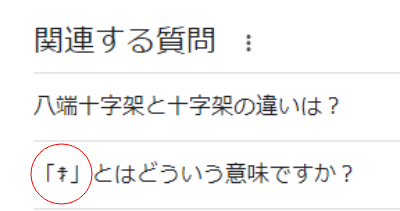
\includegraphics[width=6cm]{./images/eight-pointed-cross.png}  
\caption{「八端十字架」の Google 検索結果)}\vspace{-6mm} 
\end{figure}

  \item 正式なUnicode表記は以下となります。
\begin{figure}[H]
\centering
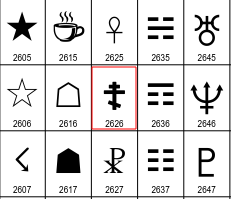
\includegraphics[width=4cm]{./images/U2626.png}  
\caption{正式なUnicode表記} 
\end{figure}
\end{itemize}
\vspace{-8mm}

\subsection*{\hspace{4mm}フォントの補正}\vspace{-2mm}
\begin{itemize}
  \item 図像を左右反転させ補正します:\bs reflectbox
\end{itemize}
\vspace{-6mm}
\begin{quote}
\begin{table}[h]
\begin{center}
\begin{tabular}{l|c|l|c}
\textbf{フォント} & \textbf{元表記} & \textbf{記述例} & \textbf{補正}\\
\hline
メイリオ(meiryo) & {\fontspec{meiryo}\fs{14}☦}(誤) & \verb+\reflectbox{\jfontspec{meiryo}+{\fontspec{meiryo}\fs{12}☦}\verb+}+ & \reflectbox{\fontspec{meiryo}{\fs{14}☦}}\\
FreeSerif & {\fontspec{FreeSerif}\fs{14}☦}(正) & \verb+{\jfontspec{FreeSerif}+{\fontspec{FreeSerif}\fs{12}☦}\verb+}+ & \\
\end{tabular}
\caption{図像の左右反転補正}\vspace{-10mm}
\end{center}
\end{table}
\end{quote}


\subsection{縦組における「…」(三点リーダー)の不具合補正}\vspace{-2mm}
% \hspace{12mm}
\begin{minipage}{12cm}
\begin{itemize}
  \item 縦組における「…」(三点リーダー)が縦組文字とならないという不具合が報告\footnotemark されています。
  \item 以下の例に示す様に文字を90度回転させるか、\textbf{全角縦三点リーダー}「︙」({\colH{800000}赤字部分=下部})を使用することでも可能です。
\end{itemize}
\end{minipage}

\vspace{-24mm}\hspace{138mm}
\vbox{\hsize=30mm\raggedright%left
\fs{14}\tate を終えた…{\colH{800000}︙}。}
% \rotatebox[origin=c]{90}{
\vspace{-10mm}
\begin{verbatim}
      を終えた\rotatebox[origin=l]{90}{…}︙。}
\end{verbatim}
\vspace{-3mm}

\footnotetext{\href{https://okumuralab.org/tex/mod/forum/discuss.php?d=3660}{LuaLaTeX縦書きでの三点リーダーが横になる} // TeX Forum 2023-11-05\\
奥村 晴彦氏の「\bs usepackage\{luatexja-preset\} を入れて、新しい `ltj-setwidth.lua` をカレントディレクトリに置くと、正常になりました」との解決法を確認しています。}

\subsection{python3.12 へのアップグレードにおける不具合 }\vspace{-2mm}
\begin{itemize}
  \item python3 (3.12.6-1) へのアップグレードにより\textbf{gedit-latex-plugins}において不具合\footnote{SyntaxWarning: invalid escape sequence}が生じています(2024-09-16)。 
  \item  これはgedit-latex-plugins側で何れ修正されると思いますが、もし問題が生じた場合は下記の対処法を試して下さい。\\ 
  \item[]\textbf{処理内容}
{\fs{5.6pt}
\begin{verbatim}
python3 (3.12.6-1) を設定しています ...
running python rtupdate hooks for python3.12...
/usr/lib/gedit/plugins/latex/latex/actions.py:254: SyntaxWarning: invalid escape sequence '\e'
  snippet_source = "\ensuremath{\mathbb{$0}}"
/usr/lib/gedit/plugins/latex/latex/actions.py:261: SyntaxWarning: invalid escape sequence '\e'
  snippet_source = "\ensuremath{\mathcal{$0}}"
/usr/lib/gedit/plugins/latex/latex/actions.py:269: SyntaxWarning: invalid escape sequence '\e'
  snippet_source = "\ensuremath{\mathfrak{$0}}"
/usr/lib/gedit/plugins/latex/latex/editor.py:146: SyntaxWarning: invalid escape sequence '\e'
  """
/usr/lib/gedit/plugins/latex/latex/expander.py:33: SyntaxWarning: invalid escape sequence '\i'
  """
/usr/lib/gedit/plugins/latex/latex/expander.py:58: SyntaxWarning: invalid escape sequence '\i'
  """
/usr/lib/gedit/plugins/latex/latex/parser.py:233: SyntaxWarning: invalid escape sequence '\e'
  """
/usr/lib/gedit/plugins/latex/latex/parser.py:509: SyntaxWarning: invalid escape sequence '\w'
  _PATTERN = compile("(TODO|FIXME)\w?\:?(?P<text>.*)")
/usr/lib/gedit/plugins/latex/latex/validator.py:40: SyntaxWarning: invalid escape sequence '\['
  """
/usr/lib/gedit/plugins/latex/preferences/__init__.py:145: SyntaxWarning: invalid escape sequence '\s'
  self._re = re.compile("^\s*%+\s*gedit:(.*)\s*=\s*(.*)")
/usr/lib/x86_64-linux-gnu/gedit/plugins/externaltools/library.py:212: SyntaxWarning: invalid escape sequence '\-'
  RE_KEY = re.compile('^([a-zA-Z_][a-zA-Z0-9_.\-]*)(\[([a-zA-Z_@]+)\])?$')
/usr/lib/x86_64-linux-gnu/gedit/plugins/snippets/substitutionparser.py:162: SyntaxWarning: invalid escape sequence '\s'
  match = re.match('\\\\?%s\s*' % self.REG_GROUP, tokens)
/usr/share/scribus/scripts/importcsv2table.py:3: SyntaxWarning: invalid escape sequence '\o'
  """
running python post-rtupdate hooks for python3.12...
\end{verbatim}
}
  \item[]\textbf{原因}\\
python3.12 において\textbf{escape sequence}の扱いが変更されたことに起因します。\\
\hspace{4mm}参照:\href{https://docs.python.org/3/whatsnew/3.12.html}{python3.12} (https://docs.python.org/3/whatsnew/3.12.html)\\
{\fs{8pt}
Other Language Changes\\
    The parser now raises SyntaxError when parsing source code containing null bytes.\\
    A backslash-character pair that is not a valid escape sequence now generates a SyntaxWarning, instead of DeprecationWarning. For \\example, re.compile("\bs d+\bs .\bs d+") now emits a \textbf{SyntaxWarning ("\bs d" is an invalid escape sequence, use raw strings for regular expression: re.compile(r"\bs d+\bs .\bs d+")).} In a future Python version, SyntaxError will eventually be raised, instead of SyntaxWarning.
}\vspace{2mm}

  \item[]\textbf{事例1:}「"」で囲まれた文字列の先頭に「{\colH{800000}r}」\footnote{raw string:バックスラッシによるエスケープシーケンスを無視し文字通りに解釈される。}を記述するか、「{\colH{800000}\bs\bs}」とします。\\
\hspace{6mm}/usr/lib/gedit/plugins/latex/latex/actions.py:254: SyntaxWarning: invalid escape sequence '\bs e'\\
\hspace{8mm}snippet\_source = "\bs ensuremath\{\bs mathbb\{\$0\}\}"\\
\hspace{8mm}修正後:{\colH{800000}r}"\bs ensuremath\{\bs mathbb\{\$0\}\}" 又は "{\colH{800000}\bs\bs}ensuremath\{{\colH{800000}\bs\bs}mathbb\{\$0\}\}"\\
% \hspace{18mm}\% 他の部分は「{\colH{800000}\bs\bs}」の記述になっていることからバグと想定されます。\\

  \item[]\textbf{事例2:}「"""」で囲まれたコメント部全体を「\#」によりコメントアウトします(上記「{\colH{800000}\bs\bs}」でも可)。\vspace{2mm}\\
\hspace{6mm}/usr/lib/gedit/plugins/latex/latex/editor.py:146: SyntaxWarning: invalid escape sequence '\bs e'\\
\hspace{8mm}"""\\\vspace{-4mm}
% \hspace{8mm}修正後:
{\fs{10pt}
\begin{verbatim}
   修正後:# """
           #  (略)
           # """
\end{verbatim}}
\end{itemize}

\newpage

\section{サンプル:トルストイ  {\fCRoman Л. Н. Толстой}}

\section{参考文献}
\printbibliography[title={参考文献(サンプル)}]
\vspace{-6mm}

\section{付録:Cyrillic Unicode表}\vspace{-2mm}
\begin{quote}
\noindent\href{https://www.unicode.org/charts/PDF/U0400.pdf}{Cyrillic: 0400–04FF}\\
\href{https://www.unicode.org/charts/PDF/U0500.pdf}{Cyrillic Supplement: 0500–052F}\\
\href{https://www.unicode.org/charts/PDF/U2DE0.pdf}{Cyrillic Extended-A: 2DE0–2DFF}\\
\href{https://www.unicode.org/charts/PDF/Unicode-15.0/U150-A640.pdf}{Cyrillic Extended-B: A640–A69F}\\
\href{https://www.unicode.org/charts/PDF/U1C80.pdf}{Cyrillic Extended-C: 1C80–1C8F}\\
\href{https://www.unicode.org/charts/PDF/U1E030.pdf}{Cyrillic Extended-D: 1E030–1E08F}\\
\end{quote}\vspace{-6mm}
\clearpage
\end{document}
